\chapter{В поисках Юрковицы}

Сейчас горой Юрковицей считают склоны от Нижнеюрковской улицы в сторону к Мыльному переулку. Прежде, пока их не сожрали многочисленные заводы, пространство горы было больше, и занимало место, вписанное, по крайней мере, во всё пространство между Нижнеюрковской, Кирилловской и упомянутым переулком. После съедения горы, между склоном и Кирилловской улицей, к нашему времени образовалась пустошь, огражденная от Кирилловской улицы промзоной (бывший кирпичный завод, бывший пивзавод и т.д.), с карьерным озером на задворках. Полоса промзоны на 2024 перестраивается в нечто иное, например в жилье.

Можно считать, что прежняя гора в этом месте практически не сохранилась, она исчезла. Остались так, крайние высоты.

Эта же гора, в 18 веке, согласно земельным документам, именовалась Лысой и, насколько можно судить, Лисавицей. Подлинники я не видел, в передаче же печатным текстом разнобой – то гора Лысая, то Лисая, я не знаю как тогда произносили, не знаю и как именно было написано. Для удобства приму название Лысая.

Известные мне документы 18 века не отражают \textbf{гору} под названием Юрковица, но есть соседствующий с Лысой Юрков ставок, из коего вытекал Юрков поток, вероятно затем преобразовавшийся в ручей Юрковицу. Насколько шаток корень привязки именования Юркова ставка водоему, изображенному на старых картах, мы разберем в отдельной главе. Ежели названия, на самом деле, при возникновении, относились к другому пруду и ручью, то многие вычисления можно смело умножить на ноль.

Сотни редких старинных карт и документов, важных для одного человека из миллиона, томятся в библиотеках и архивах, недоступные простым смертным. Я, простой смертный, могу рассуждать лишь на основании тех рукописных источников, кои пущены в обиход и которые можно рассмотреть. Например на плане конца 17 века Ушакова хоть и показаны интересующие нас склоны, имеющийся скан попросту размыт в той части (зачем тогда вообще было сканировать?), а перерисовки плана не отображают те места в нужной мере.

Доступный набор карт – а это по большому счету с середины 18 века, зачастую без легенд-объяснений – дает неоднозначную пищу для размышлений. А нам важно выяснить, где именно находилась гора Юрковица, относилось ли вообще такое название к горе, если да, то не звалась ли она в летописные времена Хоревицей.

То, что современная Юрковица не называлась в прошлом Юрковицей, доказывается хотя бы ее прежним названием – Лысая, а предшествующее имя неведомо. Однако там издавна было укрепленное поселение и массовое захоронение. Подробности поведаю позже. Там произошло нечто, после чего жизнь оттуда ушла, никто не селился. Пасли скот, гора прослыла Лысой.

Предполагаю, и по всей этой части книги поделюсь размышлениями, что на Лысой горе Кирилловских высоты стоял летописный град Киев, сооруженный Кием, Хоривом и Щеком в честь брата старшего. Каждый брат жил на своей горе-крепости отдельно. На четвертой, соседней горе, они построили общую крепость, назвав ее Киев. Чья крепость? Киева. Чей град? Киев. Это старинное склонение имени в родительном падеже. Сейчас бы сказали – град Кия, а тогда – град Киев.

Ученые никогда не рассматривали археологические находки на Лысой именно под таким углом, хотя находки эти подтверждают наличие тут древнего городища, а миниатюра из Радзивилловской летописи показывает «град Киев» здесь. Есть и другие доводы.

Но сперва кратко разберемся с обозначением горы Юрковицы и смежных с ней урочищ, важных для нас, на картах. Больше будет по мере продвижения по главам. Да, еще – иногда старинные карты нельзя точно наложить на современные, и чем глубже в прошлое, тем хуже это удается.

На плане 1752 года, показана «речка Юрковица» в пределах известного ныне в подземном коллекторе одноименного ручья, а упрощенно говоря южный склон вдоль верховий этой речки подписан «гора Щекавица». Если считать карту точной, это обозначение относится к отрогу Щекавицы, где сейчас Старообрядческое кладбище. Минусы – карта весьма условна и скорее рисует относительное расположение урочищ. Я не смог ее порядком наложить на спутник. Глубокое удолье, откуда вытекает «речка Юрковица», именуется на карте «Унизовая долина».

На весьма точном применительно к последующим векам плане Андрея Меленского 1803 года Юрковицей подписан современный угол между улицей Нижнеюрковской и Нижнеюрковским переулком. Это же место будет в разных источниках проходить как Иорданские рогатки или просто Рогатки.

%Название Юрковицы пустилось в длинное путешествие, которое надо подробно осветить. На имеющихся у меня планах Киева, с 1803 по 1865 годы, Юрковицей подписана гора, которая теперь считается отрогом Щекавицы со старообрядческим кладбищем, то бишь холм, клином вписавшийся между улицей Нижнеюрковской и Нижнеюрковским переулком. Это же место будет в разных источниках проходить как Иорданские рогатки.

На плане 1833 года «города Киева с проектом изменений», в разбираемых местах неточном, о чем можно судить по половинам Иорданского кладбища (они смещены), надпись «Юрковица» стоит поперек пруда, откуда истекает ручей. Непонятно, относится ли надпись к пруду, или склону горы. На карте 1837 года пруда уже нет, пруд был как бы сбоку общего оврага, с севера, а потом ручей стали изображать текущим из более западной точки, от нынешней котельной «Лукьяновской». Пруд же, с каких-то пор, изсчезает с карт.

На плане 1837 года «урочище Юрковица» написано внизу на упомянутом перекрестке Нижнеюрковской улицы и переулка.

План 1845 года, «урочище Юрковица» – почти там же, но ближе к Кирилловской, при этом малой частью на северо-восточном углу Щекавицы, и большей на юго-восточном углу Лысой горы между улицами Кирилловской и Нижнеюрковской. Этот еще целый, неотгрызенный склон так показателен, что приведу иллюстрацию, повернув карту на север:

\begin{center}
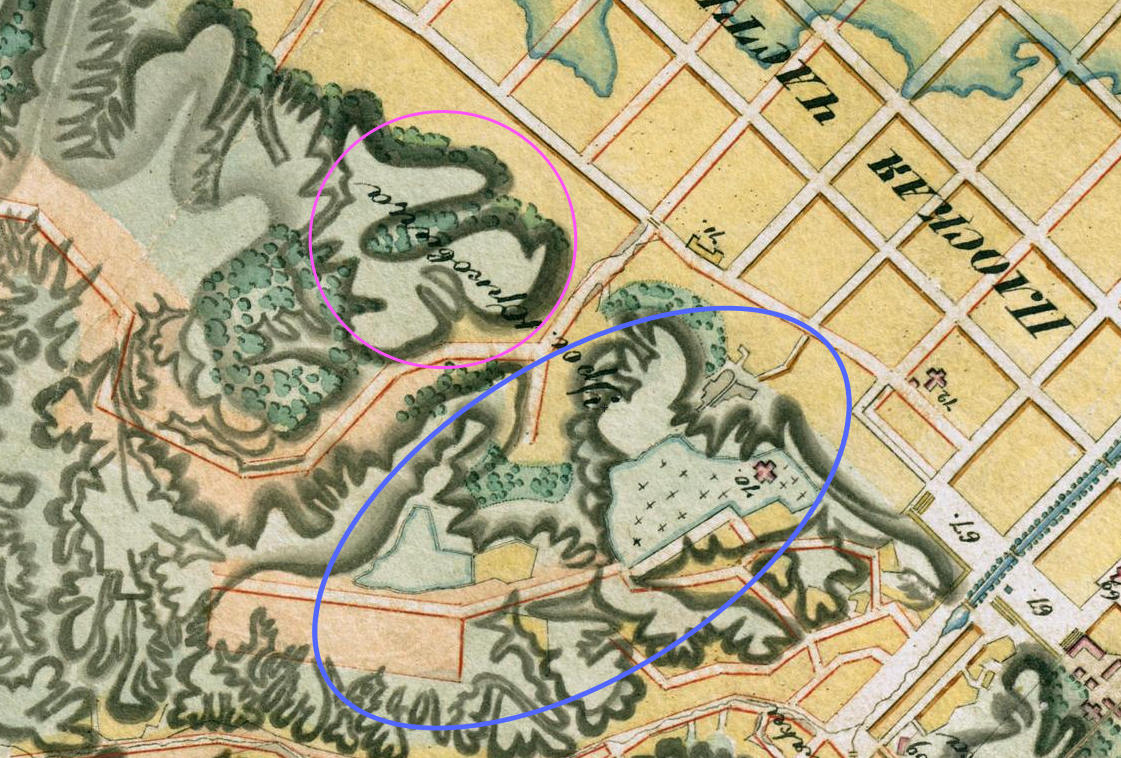
\includegraphics[width=\linewidth]{chast-kirvys/poisk-yourk/1845-marked.jpg}
\end{center} 

Синий овал – Щекавица. Розовый – подписанный как часть «уроч. Юрковица» восточный угол Лысой горы вдоль Кирилловской улицы. Как видите, гора еще существует в полной мере. Ныне там просто нет большей части горы, её съели добычей глины. Подпись же «уроч. Юрковица» начинается на противоположном склоне Щекавицы.

На великолепной карте 1847 года «урочище Юрковица» раскинулось с отрога Щекавицы где Старобрядческие кладбище, на соседний склон Лысой горы, где в яру был пруд-ставок, откуда вытекал ручей Юрковица. Если быть точным, то Старообрядческое кладбище, ежели смотреть с юга на север, лежит в начале отрога, а северная часть отрога поныне ничем не занята и хранит следы давних валов и бассейна. Вот оттуда и распростерлась надпись «урочище Юрковица». Вот этот участок, ориентировано на север, всё легко находится по сохраняющемуся поныне перекрестку – Рогаткам:

\begin{center}
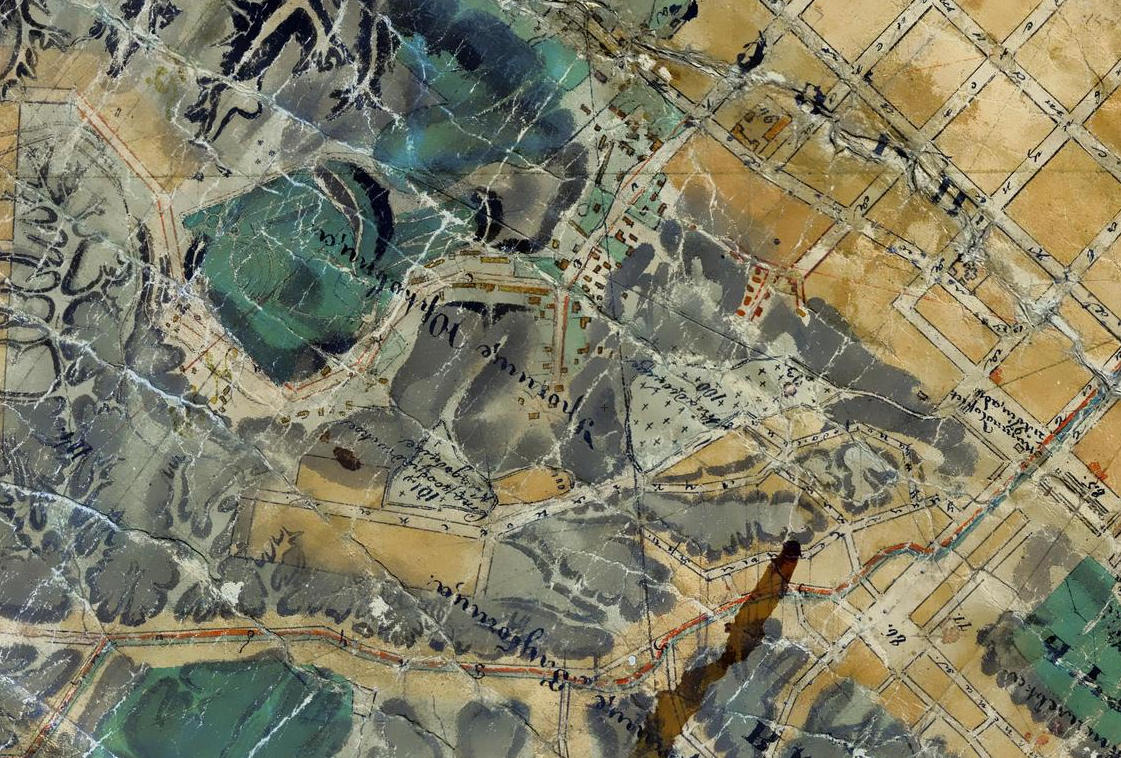
\includegraphics[width=\linewidth]{chast-kirvys/poisk-yourk/1847.jpg}
\end{center}

Уникальная карта 1860 года, где много неведомых по другим картам (подчеркиваю, картам) урочищ и есть даже Перевесище – Юрковица на повороте Нижнеюрковсой улицы в гору, затрагивает оба берега, Щекавицы и Лысой.

Карта 1861 года – та же картина. 1861 – Юрковицей подписан мыс отрога со старообрядческим кладбищем, где валы, бассейн и так далее. 1865 – то же самое.

1869 – аналогично карте 1847. 1874 – то же самое.

На карте 1880 года «Юрковица» прыгает на противоположную гору, а точнее на целый массив отрогов к северо-западу от Нижнеюрковской улицы, вдоль Кирилловской – собственно, по месту Лысой горы. То же видим на карте 1882 года из энциклопедии «Britannica», где гора подписана «Yurkova». А на замечательной в прочих отношениях карте 1886 года издания картографического заведения А. Ильина, этот же массив отрогов подписан «Щекавица». Сие повторено на французской карте 1896 года. На плане Киева с окрестностями 1909 года Лысая гора подписана Щековицей. На многих планах названий гор вообще нет, есть впрочем «Щекавицкое кладбище». На плане 1912 года мы снова видим надпись «Щекавица» там, где теперь на картах пишут «Юрковица», на Лысой.

Наконец, на последней советской карте Киева, 1991 года, Щекавица это гора, по которой идет улица Олеговская и стоит вышка. А вот «г. Юрковица» подписана к западу от «Щекавицы», та часть горы, что от Старообрядческого кладбища и в сторону котельной «Лукьяновская».

Каким образом потом, на картах и оттуда в миру, название Юрковицы переползло на бывшую Лысую гору, можно докопаться, но я не намерен этого делать.

С некоторых пор, по крайней мере допустим в 1880-е и в начале 20 века, известны улицы-урочища Нижняя Юрковица и Верхняя Юрковица, более на слуху как Нижне-Юрковская и Верхне-Юрковская. Вероятно разделение произошло, когда урочищем стало слыть большее пространство, нежели ранее. Считать давним урочищем Юрковица местности далеко от Юркового ставка – непозволительная натяжка. Однако на карте 1879 года видим огромную улицу Юрковскую от Набережно-Луговой и наверх, через всю нынешнюю Татарку до Репяхова яра, а над яром улочка Мало-Юрковская, по другими данным переулок! 

Вообще была чехарда с именованиями, они шли параллельно, например на карте одно, в адресных книгах другое.

А что полагает про Юрковицу Закревский? Наездами бывавший в Киеве и перелопативший уйму архивов. Он не пишет про такую гору.  Сначала кратко упоминает урочище Юрковицу, которое начинается в Рогатках, а затем во втором томе 1968 года издания отводит Юрковице как урочищу целую статью:

\begin{quotation}
Урочище это находится в северозападной части Киева, на том месте, где оканчивается Подол и начинается Плосское. Это есть ничто иное, как глубокий, обширный и извилистый овраг, лежащий между Скавицкими и Плосскими\footnote{Имеются в виду Кирилловские высоты.} возвышенностями. 

Узкий близ Подола овраг этот, по мере углубления в горы, разширяется и разделяется на две ветви, одна из которых левая или южная часть онаго окружена почти со всех сторон Скавикаю и составляет так называемую ближнюю Юрковицу, 
\end{quotation}

Это конечно же переулок Нижнеюрковский. Читаем далее.

\begin{quotation}
а западная или правая ветвь оврага, которая притом и длиннее, окружена с южной стороны Скавикою, а с северной стороны горой Плосскою, и составляет Дальнюю Юрковицу
\end{quotation}

Плосской горой Закревский именует Лысую гору, однако я нигде более такое название не встречал. Итак, Николай Васильевич отождествляет урочище Юрковицу с оврагом, не горой. Закревский продолжает:

\begin{quotation}
Впрочем в объявлениях иногда встречаются названия Верхней и Нижней Юрковицы. 
\end{quotation}

Далее он приводит, по его мнению, такие границы урочища Юрковица. С востока – от Плоской улицы близ Рогаток. С юга – Щековица с православным кладбищем. К западу, «на той же горе, кладбище раскольническое», к северо-западу Лукьяновка, а к северу – Иорданское кладбище. То есть Закревский продлевает урочище Юрковицу начиная от оврага современной Нижнеюровской улицы и по Иорданское кладбище, а это включает в себя современную Юрковицу.

\begin{quotation}
По дну этого урочища, собственно пространного оврага\footnote{Закревский снова сужает его до оврага.}, течет незначительный ручей Юрковица; а покатости гор в этом месте застроены, в беспорядке, небольшими деревянными домами, представляющими вид амфитеатра. Здесь же разведено несколько фруктовых садов; но по местам видны и одиноко растущие сосны\footnote{Сосны поныне растут на склоне над карьерным озером!}. Начиная от бывшей Рогатки, до западного конца в Лукьяновке, урочище это имеет в длину не более 300 сажень, а в ширину до 200, и очевидно образовалось с незапамятных времен от обвалов.

[...]

Урочище это носит название Юрковицы или Юрковки.
\end{quotation}

Я составил две карты, они на следующей странице, на коих \textbf{предполагаю} прежнее положение топонимов и показываю современное. Контуры прорисованы по немецкой аэрофотосъемке 1940-х. С тех пор мало что изменилось (кроме еще более сожранного кирпичным заводом юго-восточного склона Лысой горы), а мне было удобно, ибо на снимках четко виден рельеф.

От улицы Кирилловской на запад в овраге отходит улица Нижнеюрковская. Раньше она именовалась Большой Юрковской и просто Юрковской. С ней связана большая путаница, которой мы коснемся по мере надобности. Покамест примем, что ныне Юрковская и Нижнеюрковская делятся по соприкосновению с Кирилловской.

От Нижнеюрковской вниз, к югу, отходит Нижнеюрковский переулок, я его не подписал. Похоже на рогатку. Сия местность раньше так и называлась – Ерданские (Иорданские) Рогатки. В середине 19 века, южная ветвь их именовалась Ближней или Нижней Юрковицей, а западная – Дальней, или Верхней Юрковицей.

Сейчас все отроги горы, лежащей к югу от Нижнеюрковской улицы, считаются Щекавицей. Однако на картах первой половины 19 века, часть северо-западного отрога со старообрядческим кладбищем, дальше его к незанятому склону, иногда подписана Юрковицей. Гора напротив него, к северу, в 17-18 веках называлась Лысой. 

На моей карте овал с подписью «град Кия» не означает, что град занимал именно такое положение и имел такой размер. Скорее, град Кия покрывал всю гору.

\begin{center}
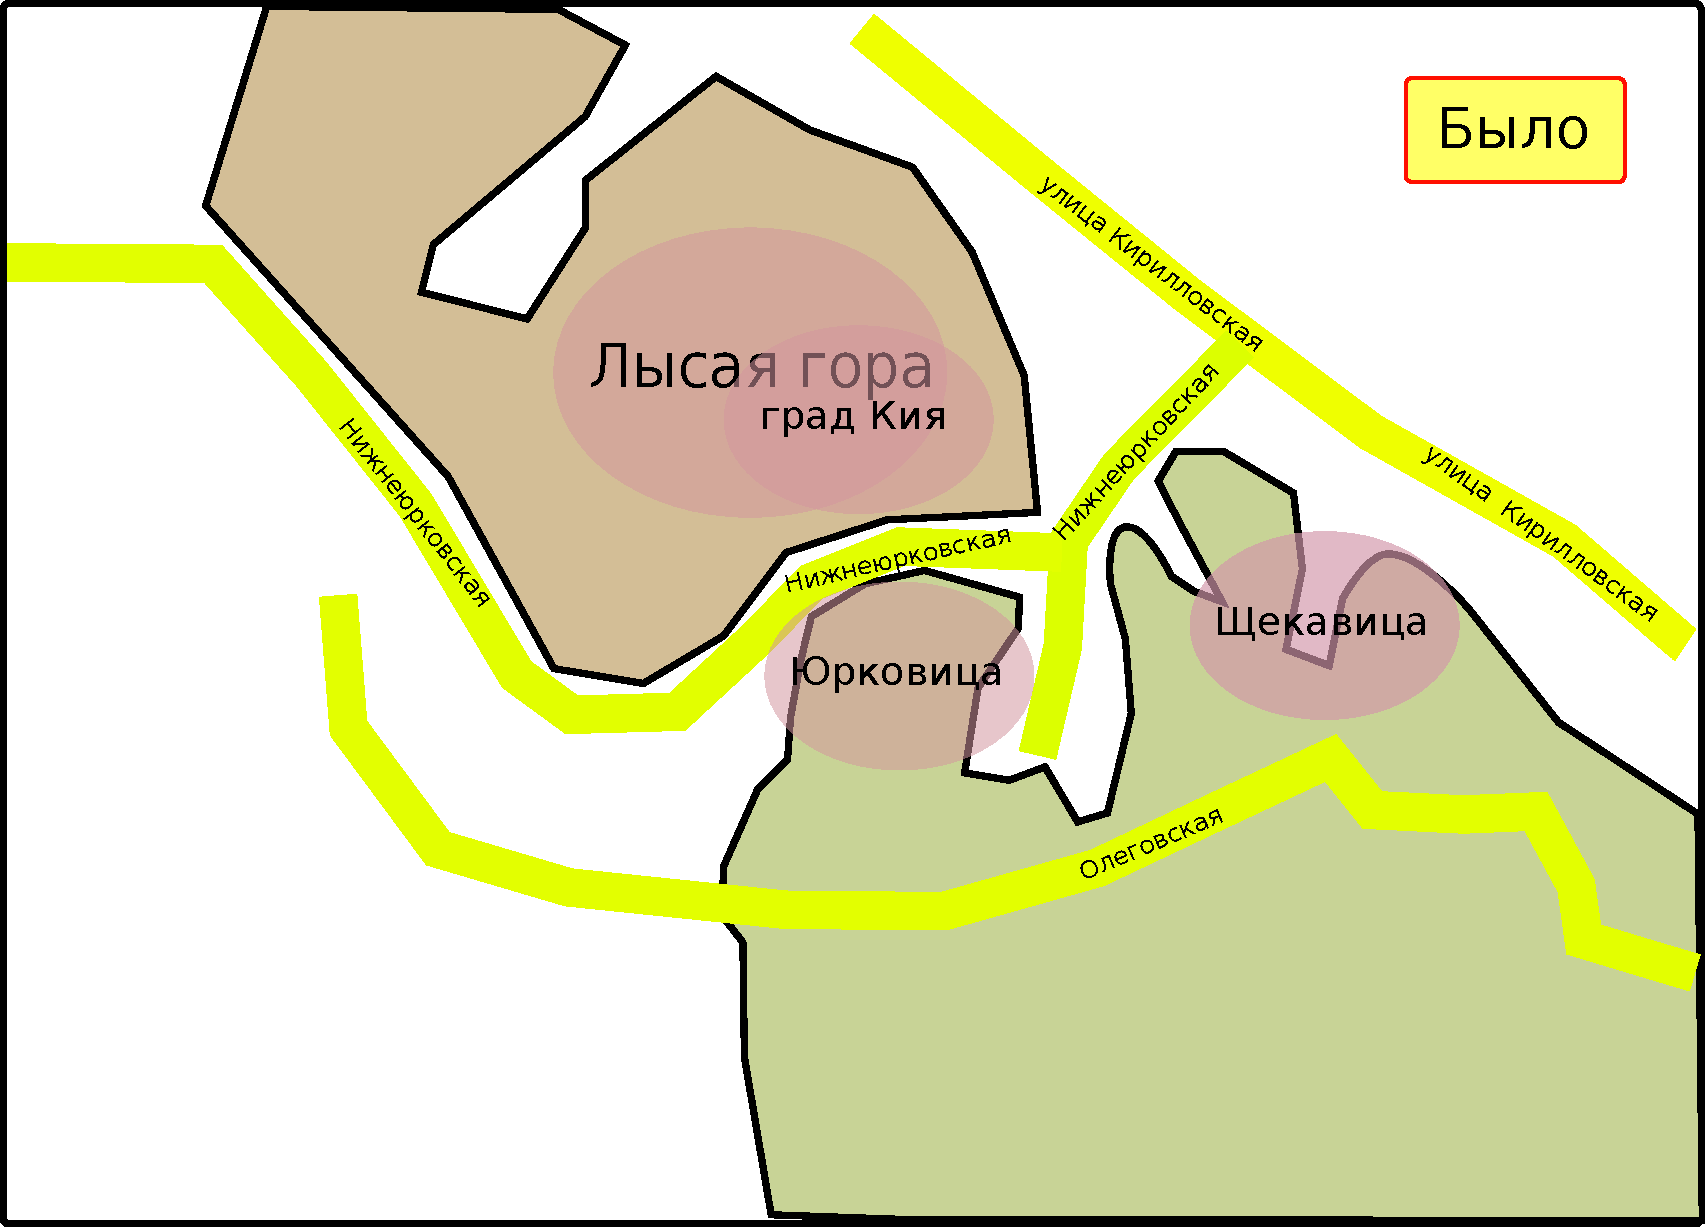
\includegraphics[width=0.90\linewidth]{chast-kirvys/poisk-yourk/yourk-bylo.pdf}
\end{center} 

\begin{center}
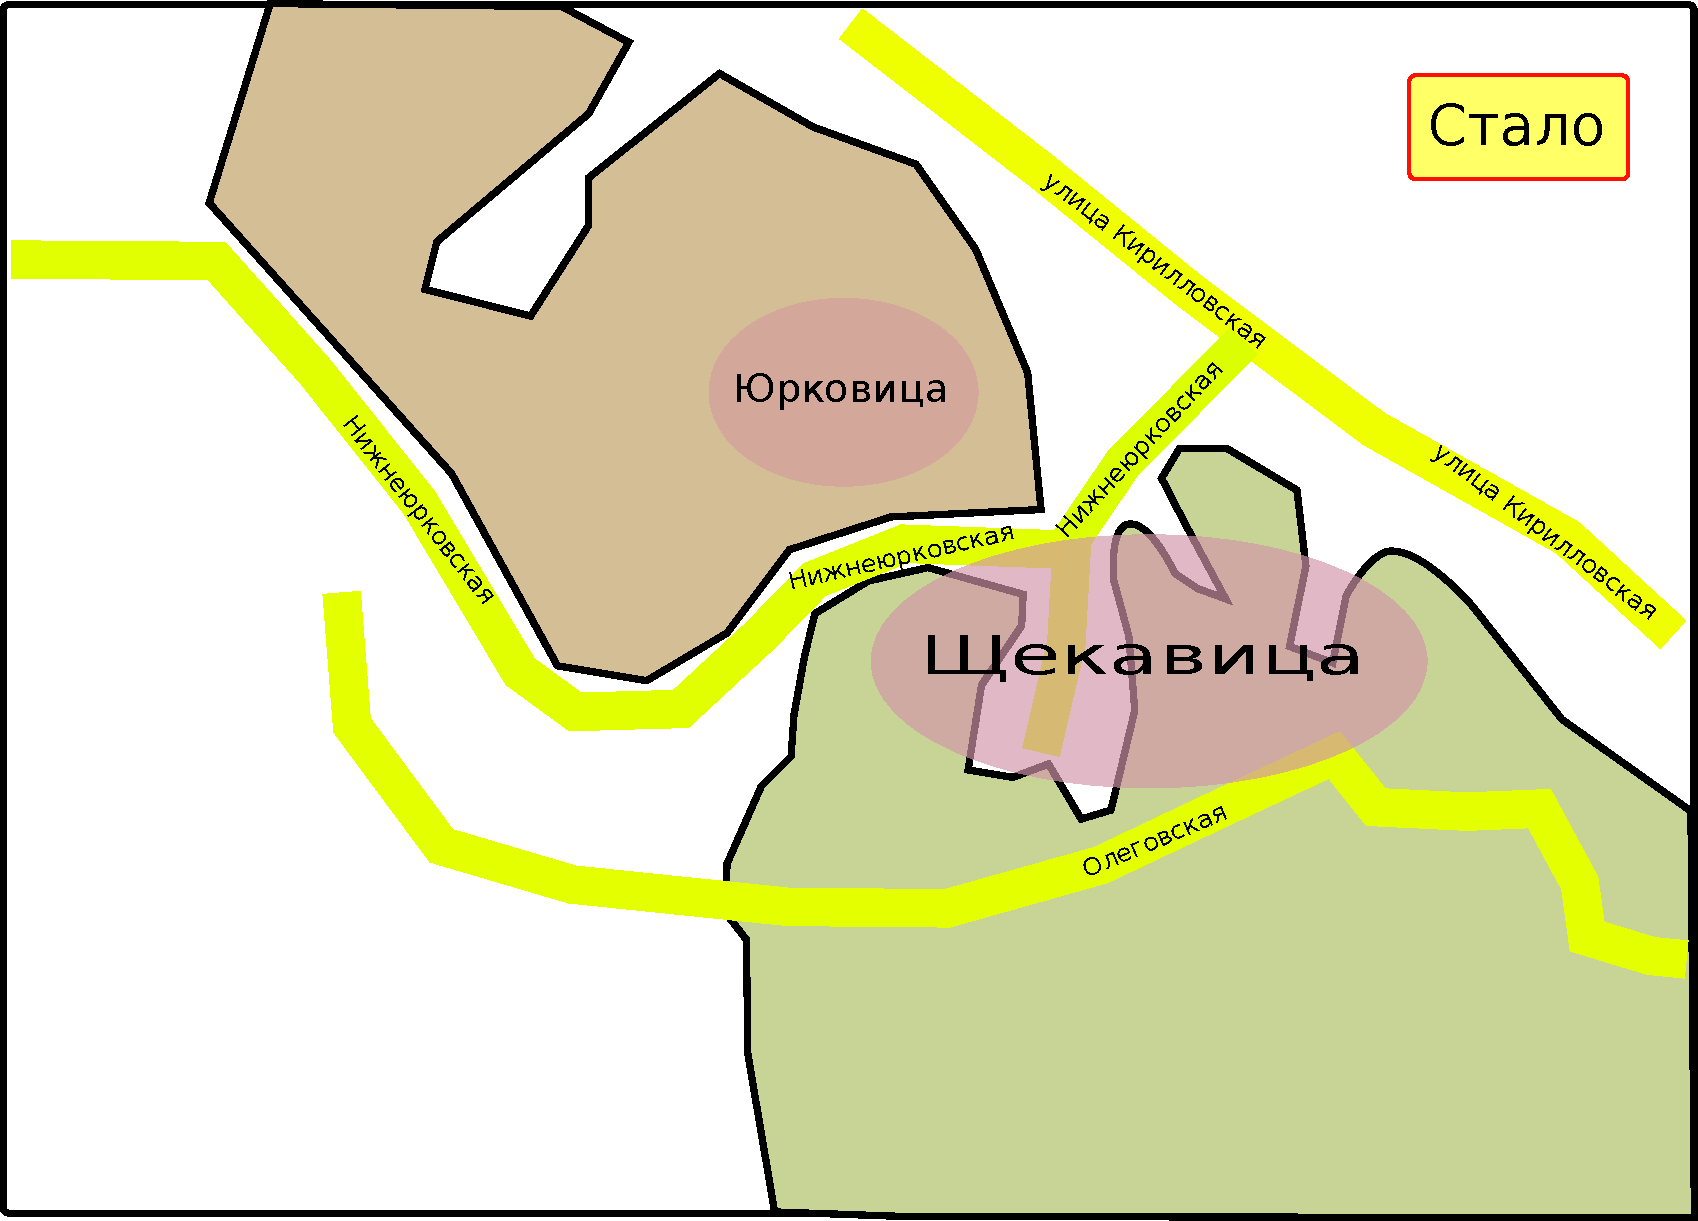
\includegraphics[width=0.90\linewidth]{chast-kirvys/poisk-yourk/yourk-stalo.pdf}
\end{center} 

Это не та гора, на которой «сидел» Кий отдельно от братьев, каждый из которых жил на своей горе, Щек на Щекавице, а Хорив на Хоривице. Овал «град Кия» это еще одна гора, где братья сообща построили крепость и нарекли ее в честь брата старшего, «град Киев».

Почему важно знать, какая гора является Юрковицей?

Здесь несколько рассуждений, от истинности или ложности которых зависит всё. Первое – Юрковица это измененное название Хоривицы, которое после летописных времен сползло вниз в урочище, и назад уже толком не вернулось. Пока утверждаю голословно.

Для удобства далее везде, где пишу про исконную гору Юрковицу, подразумеваю и Хоривицу. Ее же обозначу как Хоревица-Юрковица.

Но коль Хоривицей-Юрковицей считать Лысую гору, то «град Киев» по картинке из Радзивилловской летописи смещается дальше по Кирилловским высотам на северо-запад от Лысой.

А если полагать Хоривицей-Юрковицей гору, слывущую ныне отрогом Щекавицы со старообрядческим кладбищем, то град Кия приходится точно на бывшую Лысую гору, «новую» Юрковицу, где найдены следы древнего городища.

Вспомним еще раз миниатюру из летописи.

\begin{center}
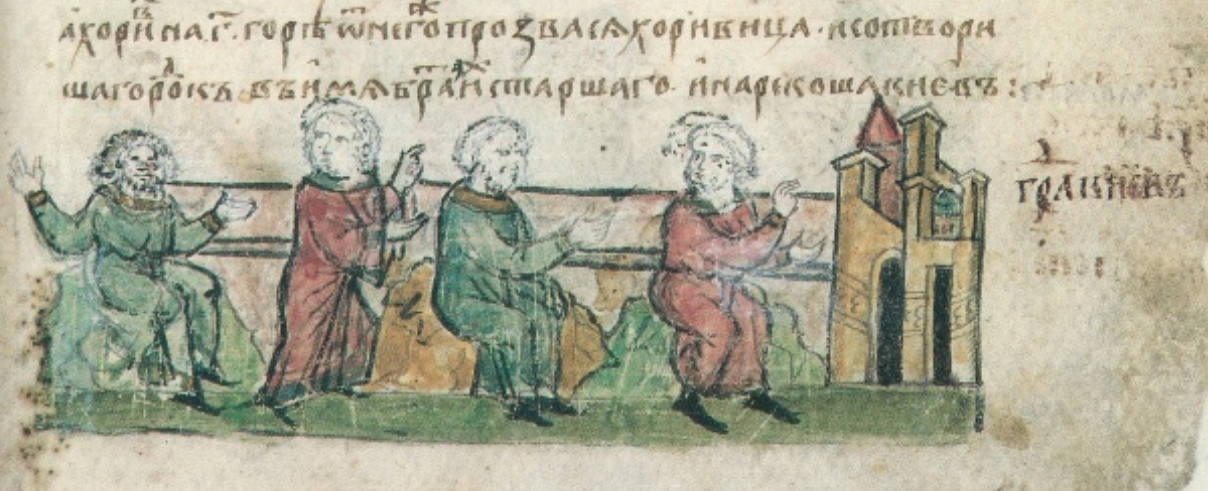
\includegraphics[width=\linewidth]{chast-kirvys/poisk-yourk/radz-tri-brata.jpg}
\end{center} 

Ежели смотреть на киевские холмы издалека с северо-востока, то третья по счету гора, Хоривица-Юрковица, на деле удалена от зрителя, в сравнении с Щекавицей и Лысой. Но художник развернул перспективу гор, поставив их на одной линии. Верно показано широкое удолье между Замковой (первая гора зеленого цвета) и Щекавицей (вторая гора, рыжая). 

Внимание! Не менее верно отражена и взаимосвязь Щекавицы с Хоривицей-Юрковицей (третьей горой, зеленой), где обе являются частями одного холма. Если бы художник хотел нарисовать справа от Щекавицы Лысую гору, он бы сделал удолье между ними глубже и шире, разделив горы. Здесь же Щекавица и Хоривица изображены соединенными, эдакая гора о двух вершинах.

В том, что иллюстрация является картой, меня убеждает и, как я уже говорил, линия реки Лыбеди на заднем плане, и кое-что другое. Зеленая равнина под холмами – ведь это Подол и Плоская часть – Оболонь!

Слева на своем холме восседает старший брат Кий. Он не выглядывает из окошка расположенного справа «града Киева». Нет, он простодушно расставил руки – радуется! Сестра Лыбедь, да братья Щек и Хорив, все указывают руками на выстроенный в честь старш\'ого град, отделенный от трех гор, справа от третьей, то бишь Хоривицы-Юрковицы.

Имя «Юрковица» переползло с одной горы на другую не только на картах.

Из материалов дела Бейлиса, которое связано с Кирилловскими высотами, явствует, что Юрковицей уже в первом десятилетии 20 века называли местность по улице Верхне-Юрковской и примыкающей к ней части улиц Половецкой, Татарской. Кажется, имя Юрковицы распространялось вместе с названиями улиц – Большая Юрковская, Верхне-Юрковская, и так далее.

Как быть дальше? Как писать дальше книгу, если под Юрковицей сейчас понимают бывшую Лысую гору, а Лысой горой считают Девич-гору за Теличкой, ниже метро «Выдубичи»?

%Нельзя говорить – это название правильное, а это нет. Название закрепилось за другой местностью в сознании не только краеведов, археологов, историков, но и местных жителей. А гора со старообрядческим кладбищем своё имя потеряла. Пустыри, заброшенные места лишаются имен, потому что людям нет смысла их вообще как-то называть.

Когда мы снимали серию «Киевской амплитуды» под названием «Возвращение в Логово змиево» и лезли на Лысую гору, то, обладая популярными знаниями, искренне считали, что поднимаемся на Юрковицу, отождествляя ее однако с летописной Хоревицей. И бродя по древнему валу, предполагали, что тут обитал Хорив. Мы-то, думаю, верно сопоставили Юрковицу с Хоревицей, просто не подозревали, что давняя Хоревица была в другом месте!

Вот карта, согласно которой я буду излагать материал, относящийся к Хоривице-Юрковице и её окрестностям. Хоривица-Юрковица там, где весь отрог со старообрядческим кладбищем. Щекавица там, где вышка, бывшая глушилка. То, что в народе слывет как «Юрковица», у меня – Лысая гора, иногда «Лысая-Юрковица».

\begin{center}
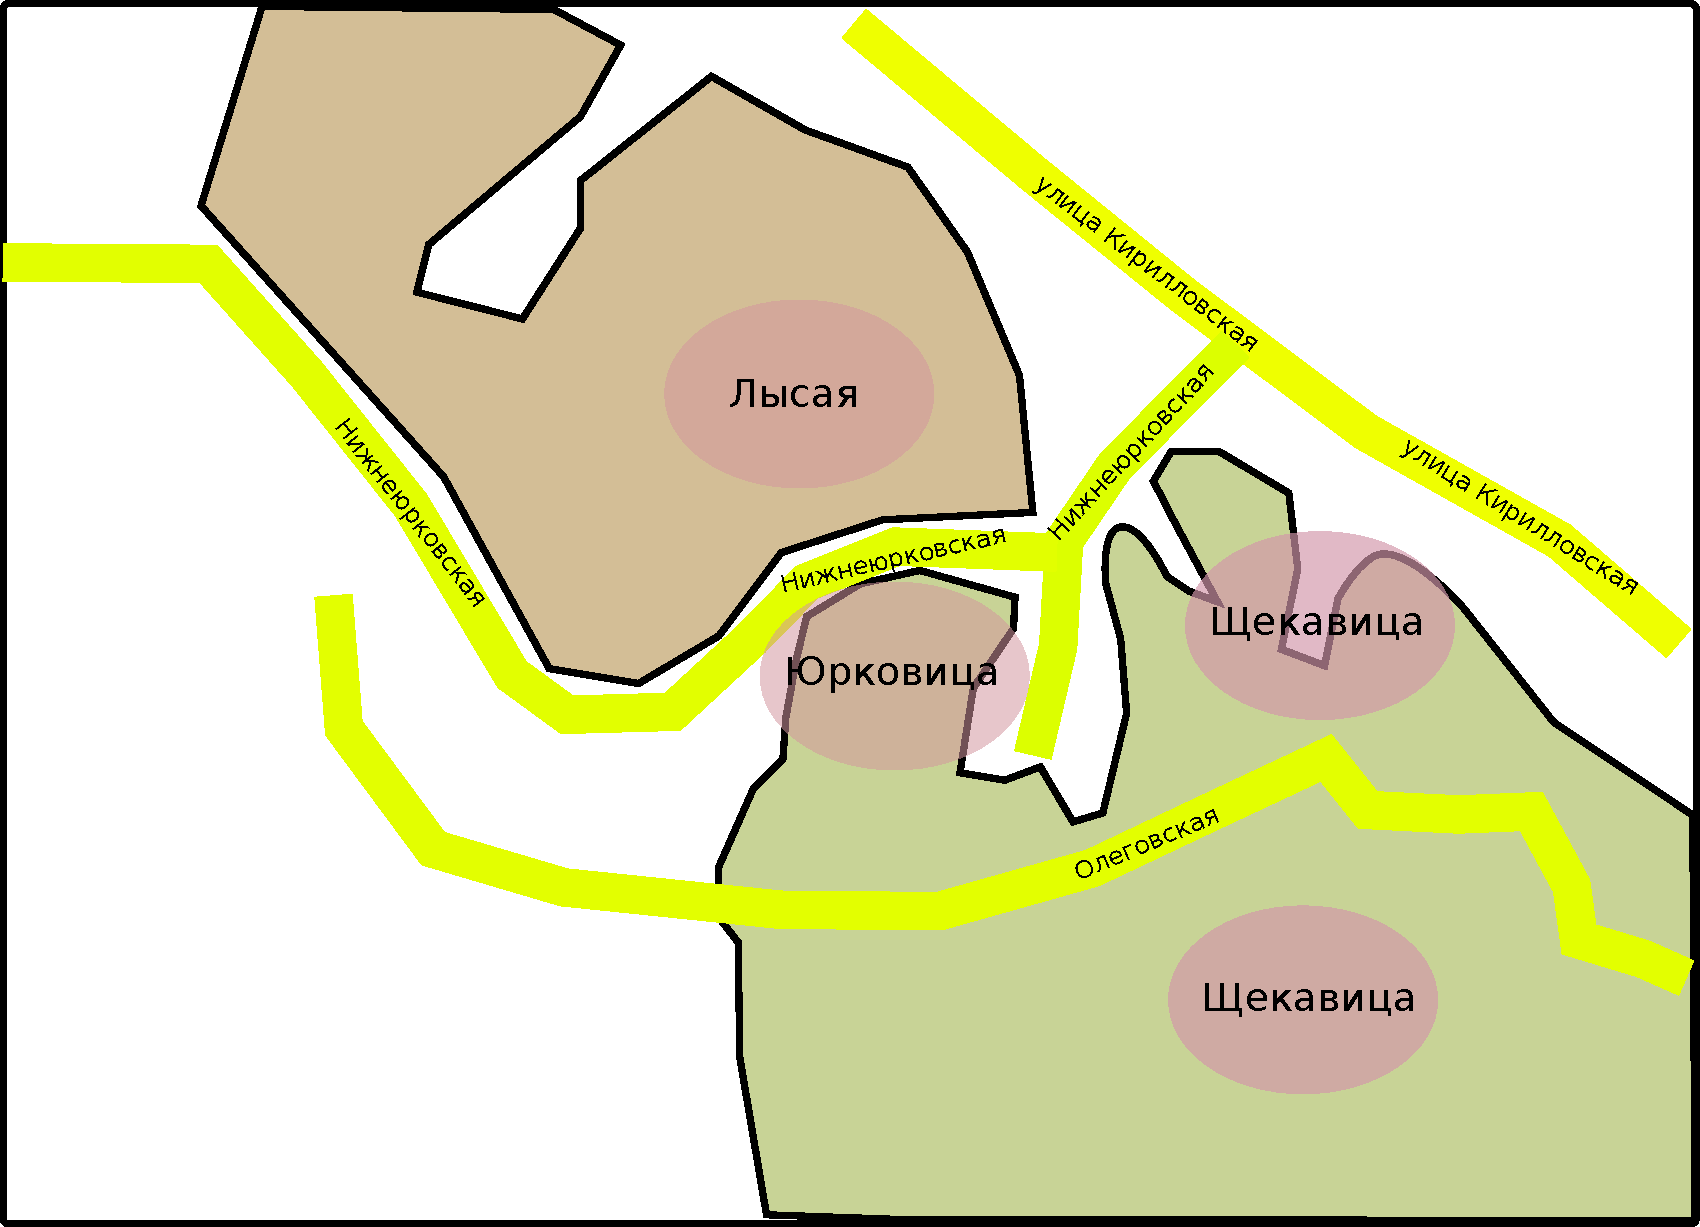
\includegraphics[width=\linewidth]{chast-kirvys/poisk-yourk/yourk-pravilno.pdf}
\end{center} 

Понимаю, что вступаю в противоречие с другими книгами и статьями про Киев. Но как быть с различными краеведческими, археологическими трудами, выходвшими в разные годы? Быть может, одни исследователи считали Юрковицей исконную Хоривицу-Юрковицу, а другие – Лысую-Юрковицу?. И поди догадайся, в чем суть, если только не дана дополнительная привязка к местности, кроме «на Юрковице».

И без того хватает путаницы и неопределенности. Само слово «Юрковица» применительно к горе отсутствует в земельных актах 17-18 веков. В документах сначала возникает, в качестве земельной межи, Юрков ставок, а не «урочище Юрковица» или целая гора. Как вы узнаете далее, положение Юркова ставка это большой вопрос, в свое время, много веков назад, решенный вероятно без оснований. Степень вероятности неизвестна.

Упоминается также, в середине 18 века, «поток Юрковиця». И потом мы видим уже урочище Юрковицу на картах 19 века, но документы с таким названием за это время мне неизвестны.

Что за Юрко или Юрий такой был, с коим связан ставок, и отсылка ли это к Хориву, или, по другому списку летописи, Оуриву, вероятно «Юрию»? 

Впрочем сомневаюсь, чтобы привязка ставка к личности сохранялась почти половину тысячелетия. С другой стороны, возможна обратная связь – от названия Хоривицы, которое с течением веков забылось, остался отголосок в имени ставка, а потом оно через ставок же возродилось, сначала как урочище, ручей и переместилось на гору, уже как «Юрковица».

Подробности об Юрковом пруде читайте в главе «Юрков ставок», там же и рассуждения о первичности названия, способные немного поколебать задачу, которую я поставил себе в этих главах.

Задача такова – обосновать, почему на Лысой горе предполагаю место града Киева. А Хоревица-Юрковица играет тут роль ориентира, смежного с градом Киевом. Все интересные находки, по которым напрашивается вывод о древнем поселении, сделаны именно на Лысой. 

И несколько смущает соседство этой Лысой горы, понимаемой мною как «град Кия», с местностью «Лукьяновка», от названия которой довольно отбросить первые две буквы, и получится «Кияновка», если вместо «кья» произносить «кия».

Одну главу я отвожу описанию исконной Хоривицы-Юрковицы. Затем мы отправимся по Лысой горе и улице Кирилловской, вдоль Кирилловских высот, с подробным разбором местности. Кирилловские высоты – уничтоженная сокровищница археологических памятников, каждый метр её уходит на тысячи лет в прошлое, а всякий замшелый кирпич или яма в земле тянет за собой переплетение историй, большей частью связанных с разрушением и смертью.

Здесь больше, чем где бы ни было в книге, я говорю о разных скелетах и костях, найденных археологами. И неожиданно поймал себя на мысли о странности в нашей системе ценностей и том, как принятое в обществе мнение об определенных вещах позволяет легко рассуждать о вещах тяжелых и обыденно воспринимать неприемлемое.

Если мы видим современную разоренную могилу, то возмущаемся вандализмом. А что раскапывают тысячи древних могил, принимается бездушно. Вроде не было таких живых людей, не носили они на шеях эти бусы, на пальцах кольца, и всё это добро их купно с останками извлекается из земли и нумеруется, заносится в каталоги, переносится в запасники различных музеев. Уважают покойников!

Завершая вводную главу про Юрковицу, не могу умолчать о неясном летописном предании. В Ипатьевском списке есть упоминание некой Серховицы, которую ученые нередко отождествляют с Юрковицей:

\begin{quotation}
6679. Сняшася братья\footnote{Союзники Андрея Боголюбского.} Вышегороде и, пришедше, сташа на Дорогожичи под святым Курилом Феодоровы недели, и второи недели оступиша весь град Киев. Мстиславу затворившюся в Киеве, бьяхуться из города, и бысть брань крепка отвсюду; Мстиславу изнемагающю в граде, Берендичи же и Торци льстяху под Мстиславом. 

И стояша 3 дни у города, и снидоша всих князий дружина Серховицею и ринушася к ним долов, у зад Мстиславу начаша стреляти. Мстиславу же начала дружина молвити: «что, княже, стоиши? поеди из города; нам их не перемочи». И поможе Бог Андреевичу Мстиславу с братьею, и взяша Киев.
\end{quotation}

Что сказано? Мстислав затворился в граде Киеве (это уже «традиционный» град Киев – Гора, там где София, Золотые ворота и так далее). И пока Мстислав сидит в городе, дружина всех князей спускается Серховицей и начинает стрелять «у зад Мстиславу».

Но ведь Мстислав – в городе, на Старокиевской горе! А где были князья до своего спуска Серховицей? На Дорогожичах под Кирилловским монастырем, а затем окружили весь Киев. И где-то в пределах окружения, сойдя Серховицей, зашли Мстиславу, который в городе, в тыл. Что же считать тылом? Тогда можно будет догадаться, что подразумевал летописец под Серховицей.

Однако надо же понимать, что спустившись по Нижнеюрковской, как думают ученые, уравнивая Серховицу и овраг по Нижнеюрковской улице, князья никак не могли стрелять «у зад Мстиславу». Но ученые не представляют себе местности или не хотят этого делать, и говорят – Серховица это Юрковица. Одни из Серховицы выкидывают буквы, другие добавляют, придумывают некое «древнерусское слово» – обычное жонглирование. 

Как по мне, что «Серховица» больше всего похоже на искаженное «Церковица». Так хотя бы осмысленно. А где она была, не знаю.
